\documentclass{article}

\usepackage{graphicx}
\usepackage{tikz}
\usepackage{tikzsymbols}
\usetikzlibrary{calc,patterns,shapes.geometric}
\pagestyle{empty}
\usepackage[margin=0pt]{geometry}
\geometry{papersize={14in,12in}}

\def\centerarc[#1](#2)(#3:#4:#5){\draw[#1] ($(#2)+({#5*cos(#3)},{#5*sin(#3)})$) arc (#3:#4:#5);}

\begin{document}
	\begin{figure}
		\centering
		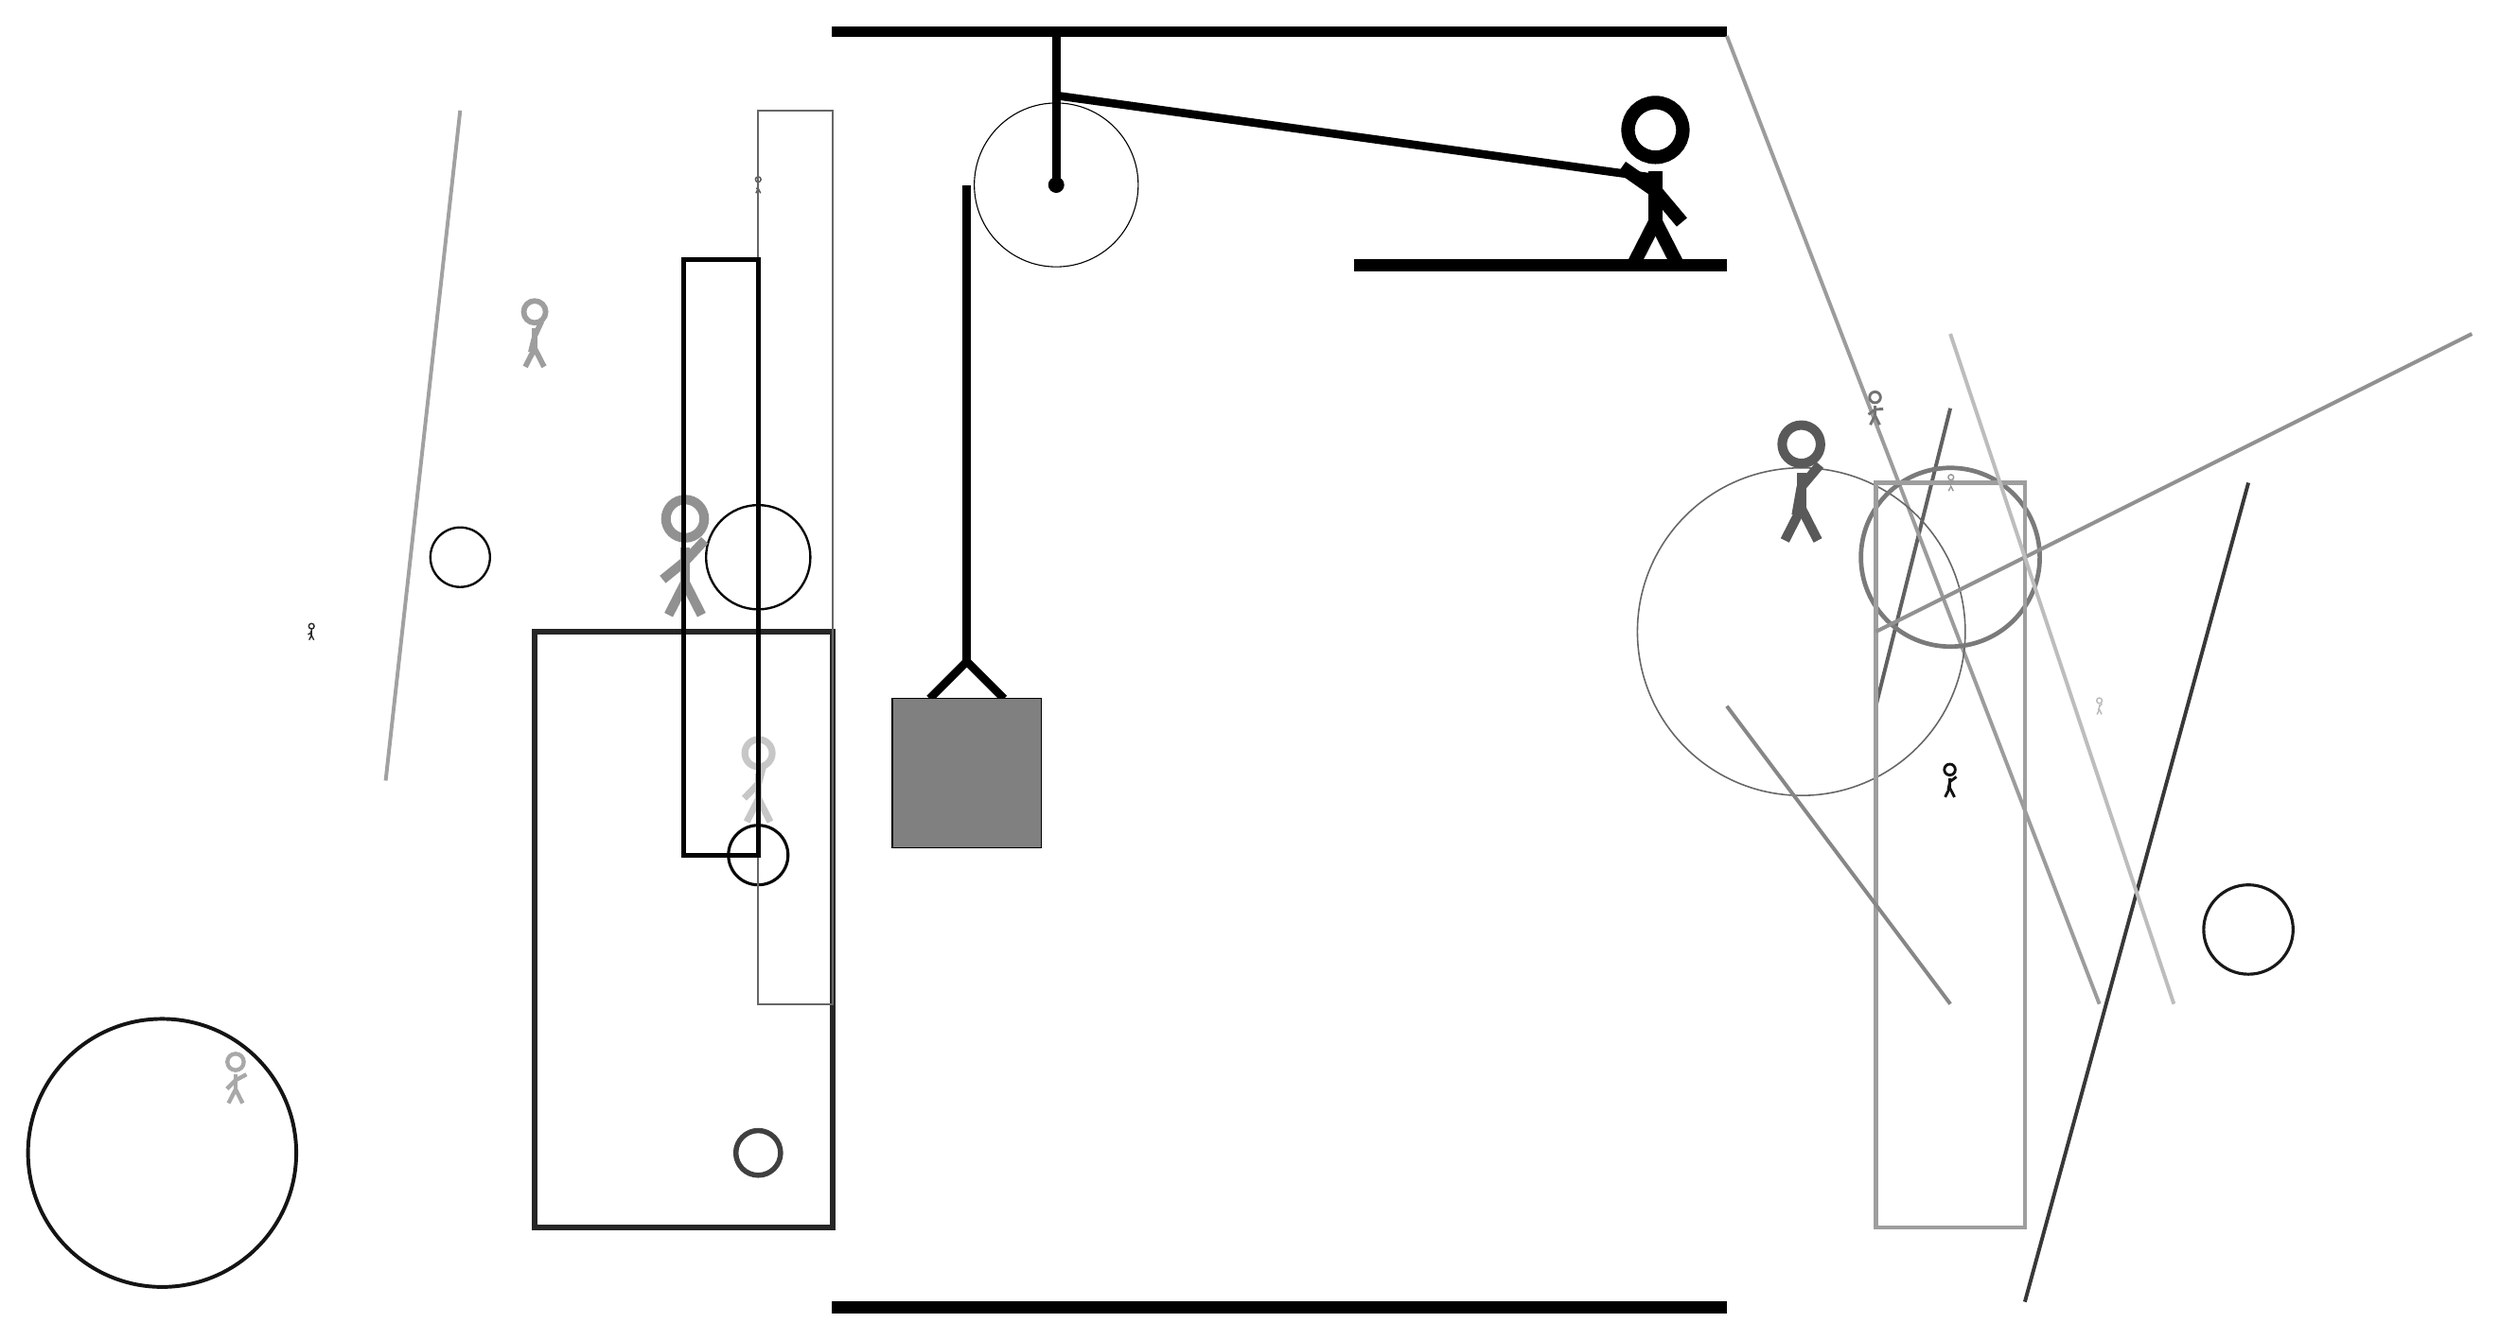
\begin{tikzpicture}
			%%%%% START %%%%%
			
			\draw[fill=black] (-2, 14) rectangle (10, 14.125);
			
			\node[line width=0.2mm, color=black!65] at (-3, 12) {\Strichmaxerl[1][67][88]};
			
			\draw[line width=0.5mm, color=black!62](12, 5) -- (13, 9);
			\draw [line width=0.3mm, color=black!97](-7, 7) circle (0.4);
			\draw [line width=0.3mm, color=black!97](-3, 7) circle (0.7);
			
			\draw [line width=0.5mm, color=black!92](-11, -1) circle (1.8);
			\node[line width=0.7mm, color=black!38] at (-6, 10) {\Strichmaxerl[4][76][65]};
			
			\draw[line width=0.5mm, color=black!39](15, 1) -- (10, 14);
			\node[line width=0.5mm, color=black!55] at (12, 9) {\Strichmaxerl[2][37][4]};
			\node[line width=0.2mm, color=black!34] at (-10, 0) {\Strichmaxerl[3][45][28]};
			
			\draw [line width=0.4mm, color=black!98](-3, 3) circle (0.4);
			\node[line width=0.7mm, color=black!22] at (-3, 4) {\Strichmaxerl[5][46][75]};
			
			\draw [line width=0.2mm, color=black!60](11, 6) circle (2.2);
			\draw [line width=0.6mm, color=black!52](13, 7) circle (1.2);
			
			\node[line width=0.7mm, color=black!83] at (-9, 6) {\Strichmaxerl[1][35][88]};
			\node[line width=0.2mm, color=black!93] at (13, 4) {\Strichmaxerl[2][79][37]};
			\draw[line width=0.6mm, color=black!38] (12, -2) rectangle (14, 8);
			\node[line width=0.3mm, color=black!65] at (11, 8) {\Strichmaxerl[7][80][50]};
			
			\draw[line width=0.7mm, color=black!85] (-2, 6) rectangle (-6, -2);
			\node[line width=0.6mm, color=black!40] at (13, 8) {\Strichmaxerl[1][16][48]};
			\draw [line width=0.7mm, color=black!75](-3, -1) circle (0.3);
			\draw[line width=0.3mm, color=black!60] (-3, 1) rectangle (-2, 13);
			
			\draw [line width=0.4mm, color=black!90](17, 2) circle (0.6);
			
			\node[line width=0.6mm, color=black!27] at (15, 5) {\Strichmaxerl[1][75][52]};
			\node[line width=0.7mm, color=black!43] at (-4, 7) {\Strichmaxerl[7][39][47]};
			\draw[line width=0.5mm, color=black!47](13, 1) -- (10, 5);
			\draw[line width=0.5mm, color=black!43](12, 6) -- (20, 10);
			\draw[line width=0.5mm, color=black!78](14, -3) -- (17, 8);
			\draw[line width=0.5mm, color=black!26](13, 10) -- (16, 1);
			
			\draw[line width=0.5mm, color=black!37](-7, 13) -- (-8, 4);
			
			\draw[line width=0.6mm, color=black!99] (-4, 3) rectangle (-3, 11);
			
			\draw (1, 12) circle (1.1);
			\draw[fill=black] (1, 12) circle (0.1);
			\draw[line width=1.1mm] (1, 14) -- (1, 12);
			
			\draw[line width=1.1mm](-0.7, 5.1) --  (-0.2, 5.6) -- (0.3, 5.1);
			\draw[fill=black!50] (-1.2, 5.1) rectangle (0.8, 3.1);
			
			\draw[line width=1.1mm](-0.2, 12) -- (-0.2, 5.6);
			\centerarc[line width=1.1mm](1, 12)(90:180:1.2000000000000002)
			\draw[line width=1.1mm](1, 13.2) -- (9, 12.1);
			
			\node at (9, 12) {\Strichmaxerl[10][-35][-50]};
			\draw[fill=black] (5, 11) rectangle (10, 10.85);
			
			\draw[fill=black] (-2, -3) rectangle (10, -3.15);
			
			%%%%% END %%%%%
		\end{tikzpicture}
	\end{figure}	
\end{document}